\documentclass[9pt,german]{beamer}%
\usepackage{master/templates/beamerthemeKIT}
\usepackage{master/templates/exercises}
\usepackage[java]{code}
\usepackage{pgfplots}
\usepackage{fontawesome}
\usepackage{ulem}

%\documentclass[9pt,trans]{beamer}%

%%%%%%%%%%%%%%%%%%%%%%%%%%%%%%%%%%%%%%%%%%%%%%%%%%%%%%%%%%%%%%%%%%%%%%%%
% Packages
%%%%%%%%%%%%%%%%%%%%%%%%%%%%%%%%%%%%%%%%%%%%%%%%%%%%%%%%%%%%%%%%%%%%%%%%
%\usepackage{beamerthemeKIT}
\usepackage[utf8]{inputenc}
% \usepackage[german]{babel}
\usepackage{helvet}
\usepackage[T1]{fontenc}
\usepackage{amsmath, amsthm, amssymb}
\usepackage{graphicx}
\usepackage{listings}
\usepackage{hyperref}
\usepackage{KITcolors}
%%%%%%%%%%%%%%%%%%%%%%%%%%%%%%%%%%%%%%%%%%%%%%%%%%%%%%%%%%%%%%%%%%%%%%%%
% Layout
%%%%%%%%%%%%%%%%%%%%%%%%%%%%%%%%%%%%%%%%%%%%%%%%%%%%%%%%%%%%%%%%%%%%%%%%
\renewcommand{\rmdefault}{phv}
\newlength{\movetitlegrafics}
\setlength{\movetitlegrafics}{0.0\paperwidth}
%%%%%%%%%%%%%%%%%%%%%%%%%%%%%%%%%%%%%%%%%%%%%%%%%%%%%%%%%%%%%%%%%%%%%%%%
% Definitions
%%%%%%%%%%%%%%%%%%%%%%%%%%%%%%%%%%%%%%%%%%%%%%%%%%%%%%%%%%%%%%%%%%%%%%%%
%%% Counter
\newcounter{ctlit}%
\setcounter{ctlit}{1}%
\newcounter{kap}

%%% Textfarben
\newcommand\BLUE[1]{\textcolor{KITblue}{#1}}%
\newcommand\BLACK[1]{\textcolor{KITblack}{#1}}%
\newcommand\GREEN[1]{\textcolor{KITgreen}{#1}}%
\newcommand\LBLUE[1]{\textcolor{KITblue15}{#1}}%
\newcommand\RED[1]{\textcolor{KITred}{#1}}%
%%% Layout
\def\cmt#1{\BLUE{#1}}%
\def\code#1{\texttt{#1}}%
\def\codeblock#1{\GREEN{\texttt{#1}}}%
\def\ftext#1{\textbf{{#1}}}%
\def\headline#1{\large\textbf{\GREEN{#1}}}%
\def\KITitem{\KITBullet[2mm]\ }%
\def\q{\quad}%
\def\qq{\qquad}%
\def\subtitle#1{{\small #1}}%
\def\tab{\hspace*{0.5cm}}%
%%% Standards
%\input{D:/TeX/formate/mystyle/defs}%
%\input{/home/ae01/tex/formate/mystyle/defs}%
%%% Text
%%% Symbols
\def\bs{$\backslash$}%
\def\hpm{\hphantom{$-$}}%
\def\meps{\epsilon}%
%%% code environment
\lstset{
  showstringspaces=false,
  numbers=none,
  keywordstyle=\color{KITgreen},  % coloring and formatting of keywords as public, class, import 
  commentstyle=\color{KITblue}\small\ttfamily, % Color of comments
  stringstyle=\color{KITred},
  breaklines=true
}

\lstdefinestyle{JAVA}
{
  language=Java,
  basicstyle=\ttfamily, % defines text formatting
  frame=tb  % print top and bottom lines, frame=single, L
}

\lstdefinestyle{JAVAsmall}
{
  language=Java,
  basicstyle=\small\ttfamily, % defines text formatting
  frame=tb  % print top and bottom lines, frame=single, L
}

\lstdefinestyle{JAVAlines}
{
  language=Java,
  numbers=left,
  numberstyle=\color{KITblack50}\ttfamily,
  numbersep=4pt, % distance between numbers and code1_1
  xleftmargin=4pt, % distance from frame to listing
  xrightmargin=4pt, % distance from frame to listing
  basicstyle=\ttfamily, % defines text formatting
  keywordstyle=\color{KITgreen},  % coloring and formatting of keywords as public, class, import 
  commentstyle=\color{KITblue}\ttfamily, % Color of comments
  frame=tb  % print top and bottom lines, frame=single, L
}

\lstdefinestyle{JAVAsmalllines}
{
  language=Java,
  numbers=left,
  numberstyle=\color{KITblack50}\ttfamily,
  numbersep=4pt, % distance between numbers and code1_1
  xleftmargin=4pt, % distance from frame to listing
  xrightmargin=4pt, % distance from frame to listing
  basicstyle=\small\ttfamily, % defines text formatting
  keywordstyle=\color{KITgreen},  % coloring and formatting of keywords as public, class, import 
  commentstyle=\color{KITblue}\ttfamily, % Color of comments
  frame=tb  % print top and bottom lines, frame=single, L
}


\lstdefinestyle{BASH}{
  basicstyle=\Large\ttfamily, % defines text formatting
  frame=none,
  language=bash
}


%%%%%%%%%%%%%%%%%%%%%%%%%%%%%%%%%%%%%%%%%%%%%%%%%%%%%%%%%%%%%%%%%%%%%%%%
% Titlepage
%%%%%%%%%%%%%%%%%%%%%%%%%%%%%%%%%%%%%%%%%%%%%%%%%%%%%%%%%%%%%%%%%%%%%%%%
\title[Institut f\"ur Angewandte und Numerische Mathematik]%
 {\fontsize{15}{15}\selectfont{}
  \"Ubung:
  \textit{Einstieg in die Informatik}\\[1.5mm]
  \textit{\phantom{\"Ubung:}\; und algorithmische Mathematik}\\[1.5mm]
  }%\hspace*{3cm}\normalsize{f\"ur Mathematiker}}
\author{\fontsize{9}{9}\selectfont{}
 Albert Mink\
  }
\institute[Institut f\"ur Angewandte und Numerische Mathematik]
 {\fontsize{6}{6}\selectfont{}%
  Institut f\"ur Angewandte und Numerische Mathematik}
\date{Wintersemester 2018/19}%
\subject{}%
%\beamerdefaultoverlayspecification{<+->}
%%%%%%%%%%%%%%%%%%%%%%%%%%%%%%%%%%%%%%%%%%%%%%%%%%%%%%%%%%%%%%%%%%%%%%%%



\makeatletter
\def\input@path{{uebungsfolien/}}
\graphicspath{{uebungsfolien/}}
\makeatother


%%%%%%%%%%%%%%%%%%%%%%%%%%%%%%%%%%%%%%%%%%%%%%%%%%%%%%%%%%%%%%%%%%%%%%%%
% Document
%%%%%%%%%%%%%%%%%%%%%%%%%%%%%%%%%%%%%%%%%%%%%%%%%%%%%%%%%%%%%%%%%%%%%%%%
\begin{document}
\maketitle%
\addtocounter{framenumber}{-1}%
%%%%%%%%%%%%%%%%%%%%%%%%%%%%%%%%%%%%%%%%%%%%%%%%%%%%%%%%%%%%%%%%%%%%%%%%


%%%%%%%%%%%%%%%%%%%%%%%%%%%%%%%%%%%%%%%%%%%%%%%%%%%%%%%%%%%%%%%%%%%%%%%%
%%%%%%%%%%%%%%%%%%%%%%%%%%%%%%%%%%%%%%%%%%%%%%%%%%%%%%%%%%%%%%%%%%%%%%%%
\begin{frame}
  \frametitle{Arbeitsblatt 3}%
\tableofcontents[hideallsubsections]
\end{frame}
\setcounter{exercise}{8}
%%%%%%%%%%%%%%%%%%%%%%%%%%%%%%%%%%%%%%%%%%%%%%%%%%%%%%%%%%%%%%%%%%%%%%%%



%%%%%%%%%%%%%%%%%%%%%%%%%%%%%%%%%%%%%%%%%%%%%%%%%%%%%%%%%%%%%%%%%%%%%%%%
%%%%%%%%%%%%%%%%%%%%%%%%%%%%%%%%%%%%%%%%%%%%%%%%%%%%%%%%%%%%%%%%%%%%%%%%
\section{Wiederholung}\label{K:wdh}
\begin{frame}
  \frametitle{\ref{K:wdh} Wiederholung}%
\tableofcontents[current]
\end{frame}
%%%%%%%%%%%%%%%%%%%%%%%%%%%%%%%%%%%%%%%%%%%%%%%%%%%%%%%%%%%%%%%%%%%%%%%%


%%%%%%%%%%%%%%%%%%%%%%%%%%%%%%%%%%%%%%%%%%%%%%%%%%%%%%%%%%%%%%%%%%%%%%%%
%%%%%%%%%%%%%%%%%%%%%%%%%%%%%%%%%%%%%%%%%%%%%%%%%%%%%%%%%%%%%%%%%%%%%%%%
\def\stitle{Beachtung der Priorit\"at}
\subsection{\stitle}\label{S:Priorit\"at}
\begin{frame}[fragile]%
  \frametitle{\ref{K:wdh}.\ref{S:Priorit\"at} \stitle}%
\medskip

Gegeben sei der folgende Java--Ausdruck:
\begin{center}
\code{a || b \&\& c}
\end{center}
Dabei seien \code{a, b, c} Variablen vom Typ \code{boolean}.
\medskip

Wie wird dieser Ausdruck abgearbeitet (engl. \emph{operator precedence})?
\begin{itemize}
  \item [a)] \code{(a || b) \&\& c}
  \item[b)] \code{a || b( \&\& c)}
\end{itemize}

Welche der folgenden Ausdr\"ucke ist die korrekte \textbf{Negation}?
\begin{itemize}
  \item [a)] \code{!a \&\& (!b || !c)}
  \item [b)] \code{!a \&\& \ !b || !c}
\end{itemize}

\end{frame}
%%%%%%%%%%%%%%%%%%%%%%%%%%%%%%%%%%%%%%%%%%%%%%%%%%%%%%%%%%%%%%%%%%%%%%%%


%%%%%%%%%%%%%%%%%%%%%%%%%%%%%%%%%%%%%%%%%%%%%%%%%%%%%%%%%%%%%%%%%%%%%%%%
%%%%%%%%%%%%%%%%%%%%%%%%%%%%%%%%%%%%%%%%%%%%%%%%%%%%%%%%%%%%%%%%%%%%%%%%
\def\stitle{Offizielle Dokumentation}
\subsection{\stitle}\label{S:Dokumentation}
\begin{frame}[fragile]%
  \frametitle{\ref{K:wdh}.\ref{S:Dokumentation} \stitle}%
%%source
\url{docs.oracle.com/javase/tutorial/java/nutsandbolts/operators.html}

\begin{center}
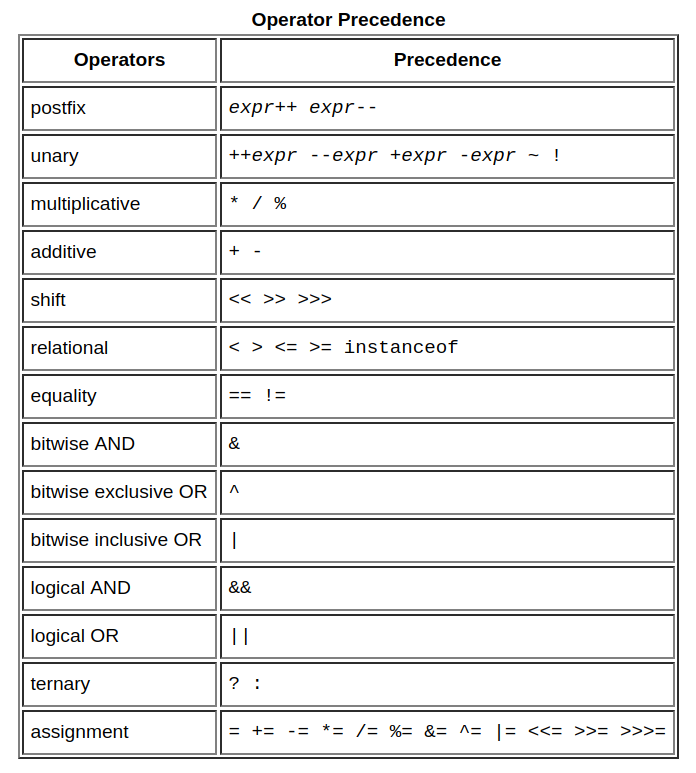
\includegraphics[width=0.6\textwidth]{grundl-boolalgnegation/operatorPrecedence}
\end{center}
\end{frame}
%%%%%%%%%%%%%%%%%%%%%%%%%%%%%%%%%%%%%%%%%%%%%%%%%%%%%%%%%%%%%%%%%%%%%%%%


%%%%%%%%%%%%%%%%%%%%%%%%%%%%%%%%%%%%%%%%%%%%%%%%%%%%%%%%%%%%%%%%%%%%%%%%
%%%%%%%%%%%%%%%%%%%%%%%%%%%%%%%%%%%%%%%%%%%%%%%%%%%%%%%%%%%%%%%%%%%%%%%%
\def\stitle{De Morgansche Gesetze}
\subsection{\stitle}\label{S:Morgansche}
\begin{frame}[fragile]%
  \frametitle{\ref{K:wdh}.\ref{S:Morgansche} \stitle}%
Vergleich Analysis I
\medskip

\begin{description}
  \item[und bzw. oder]
  \item $\neg \neg A = A$
  \item $\neg (A \wedge B) = \neg A \vee \neg B$
  \item $\neg (A \vee B) = \neg A \wedge \neg B$
\end{description}
\medskip

\begin{description}
  \item[Schnittmenge bzw. Vereinigung]
  \item $(A^{\mathsf{c}})^{\mathsf{c}} = A$
  \item $(A \cap B)^{\mathsf{c}} = A^{\mathsf{c}} \cup B^{\mathsf{c}}$
  \item $(A \cup B)^{\mathsf{c}} = A^{\mathsf{c}} \cap B^{\mathsf{c}}$
\end{description}

\end{frame}
%%%%%%%%%%%%%%%%%%%%%%%%%%%%%%%%%%%%%%%%%%%%%%%%%%%%%%%%%%%%%%%%%%%%%%%%

\begin{frame}[t]%
\medskip

\begin{exercise}{Boolsche Algebra}
\begin{body}
Unter der Negation eines Boolschen Ausdrucks $A$ versteht man den Ausdruck $\neg A$. Dieser ist genau dann wahr, wenn $A$ falsch ist. Seien $A$ und $B$ Boolsche Ausdrücke, so gelten die folgenden Negationsregeln
\begin{align*}
\neg \neg A &= A,\\
\neg (A \wedge B) &= \neg A \vee \neg B,\\
\neg (A \vee B)   &= \neg A \wedge \neg B. \\
\end{align*}
Geben Sie die \textbf{Negation} der nachfolgenden Java--Ausdrücke jeweils als Java--Ausdruck an. Hierbei seien \code{a} und \code{b} Variablen vom Typ \code{int}.\\[1em]
\begin{center}
\begin{minipage}{0.35\textwidth}
\begin{itemize}
\item[(a)] \code{a == 1}
\item[(b)] \code{(a == 1) || (b == 2)}
\item[(c)] \code{(a >= 0) \&\& (a <= 1)}
\end{itemize}
\end{minipage}
\quad
\begin{minipage}{0.6\textwidth}
\begin{itemize}
\item[(d)] \code{(a != 1) || (b == 4)}
\item[(e)] \code{(a != 0) \&\& (a != 1) \&\& (a != 2)}
\item[(f)] \code{(b < -1) || (b > 1) || (a == 0)}
\end{itemize}
\end{minipage}
\end{center}
\end{body}
\end{exercise}

\end{frame}
%%%%%%%%%%%%%%%%%%%%%%%%%%%%%%%%%%%%% solution %%%%%%%%%%%%%%%%%%%%%%%%%%%%%%%%%%%%%%%%%%%%%%%%%%%%%%%%%%%%%%%
% \begin{solution}
% \begin{center}
% \begin{minipage}{0.45\textwidth}
% \begin{itemize}
% \item[(a)] a!=1
% \item[(b)] \code{(a != 1) && (b != 2)}
% \item[(c)] \code{(a < 0) || (a > 1)}
% \end{itemize}
% \end{minipage}
% \begin{minipage}{0.45\textwidth}
% \begin{itemize}
% \item[(d)] \code{(a == 1) && (b != 4)}
% \item[(e)] \code{(a == 0)||(a == 1)||(a == 2)}
% \item[(f)] \code{(b >= -1) && (b <= 1) && (a != 0)}
% \end{itemize}
% \end{minipage}
% \end{center}
% \end{solution}

\section{Aufgabe 14}
\def\stitle{\theexercise\ - Anweisungen 1}
\section{\stitle}
\begin{frame}[t]%
    \frametitle{\stitle}

Gegeben sei der folgende Ausschnitt eines Java-Programms. Sei \code{n} vom Typ \code{int}.

\lstinputlisting[style=JAVAsmalllines]{anweis-1/Anweis1_snippet.java}

\begin{itemize}
\item[a)] Welcher Buchstabe wird auf dem Bildschirm ausgegeben, falls \code{n} den Wert $1$, $2$, $3$ bzw. $4$ besitzt?
\end{itemize}
\end{frame}


%%%%%%%%%%%%%%%%%%%%%%%%%%%%%%%%%%%%%%%%%%%%%%%%%%%%%%%%%%%%%%%%%%%%%%%%
\begin{frame}[fragile]%
 \frametitle{a) Struktogramm mit Java-Editor}%

\begin{center}
\lstinputlisting[style=JAVAlines]{anweis-1/Anweis1_snippet.java}
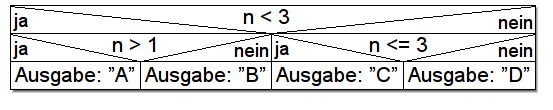
\includegraphics[width=0.8\textwidth]{anweis-1/Bilder/Struktogramm_a}
\end{center}

\end{frame}

\begin{frame}[t]%
    \frametitle{\stitle}

Gegeben sei der folgende Ausschnitt eines Java-Programms. Sei \code{n} vom Typ \code{int}.

\lstinputlisting[style=JAVAsmalllines]{anweis-1/Anweis1_snippet.java}

\begin{itemize}
\item[b)] Welcher Buchstabe wird auf dem Bildschirm ausgegeben, falls \code{n} den Wert $1$, $2$, $3$ bzw. $4$ besitzt und \textbf{jeder} Boolsche Ausdruck in dem Programmabschnitt durch seine Negation ersetzt wurde?
\end{itemize}
\end{frame}

%%%%%%%%%%%%%%%%%%%%%%%%%%%%%%%%%%%%%%%%%%%%%%%%%%%%%%%%%%%%%%%%%%%%%%%%
\begin{frame}[fragile]%
\frametitle{b) Strukturprogramm mit Java-Editor}%
\begin{center}
\lstinputlisting[style=JAVAlines]{anweis-1/Anweis1_snippet.java}
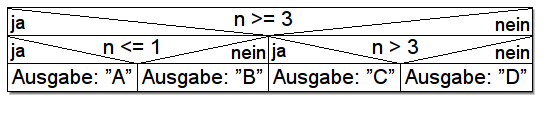
\includegraphics[width=0.8\textwidth]{anweis-1/Bilder/Struktogramm_b}
\end{center}

\end{frame}


%%%%%%%%%%%%%%%%%%%%%%%%%%%%%%%%%%%%%%%%%%%%%%%%%%%%%%%%%%%%%%%%%%%%%%%%
\begin{frame}[fragile]%
 \frametitle{c) Beispiel Programm}%
\lstinputlisting[style=JAVAsmall, basicstyle=\footnotesize\ttfamily]{anweis-1/Anweis1.java}
\end{frame}

%%%%%%%%%%%%%%%%%%%%%%%%%%%%%%%%%%%%%%%%%%%%%%%%%%%%%%%%%%%%%%%%%%%%%%%%
%%%%%%%%%%%%%%%%%%%%%%%%%%%%%%%%%%%%%%%%%%%%%%%%%%%%%%%%%%%%%%%%%%%%%%%%
\def\stitle{Wdh. Typumwandlung}
\subsection{\stitle}\label{S:Typumwandlung}
\begin{frame}[fragile]%
  \frametitle{\ref{K:wdh}.\ref{S:Morgansche} \stitle}%
\medskip

Allgemein \code{(Datentyp)(Ausdruck)}.
\lstinputlisting[style=JAVAlines]{typumwandung/Typumwandlung.java}

\end{frame}
%%%%%%%%%%%%%%%%%%%%%%%%%%%%%%%%%%%%%%%%%%%%%%%%%%%%%%%%%%%%%%%%%%%%%%%%
\section{Aufgabe 15}
\def\stitle{\theexercise\ - Anweisungen 2}
\section{\stitle}
\begin{frame}[t]%
    \frametitle{\stitle}

Gegeben sei der folgende Ausschnitt eines Java-Programms.
\lstinputlisting[style=JAVAsmalllines]{anweis-2/Anweis2.java}

\begin{itemize}
\item[(a)] Welcher Buchstabe wird auf dem Bildschirm ausgegeben, falls \code{i} den Wert $1$, $2$, $3$ bzw. $4$ besitzt?
\item[(b)] Realisieren Sie diesen Programmausschnitt mit einer \code{switch}-Anweisung.
\end{itemize}
\end{frame}


\begin{frame}[fragile]%
 \frametitle{a) Strukturprogramm mit Java-Editor}%

\begin{center}
\lstinputlisting[style=JAVAlines]{anweis-2/Anweis2_snippet.java}
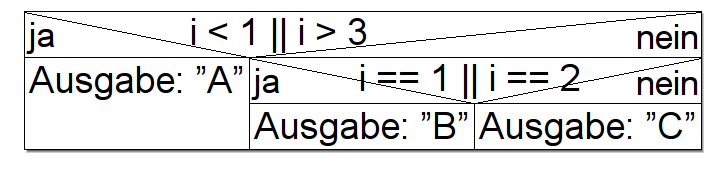
\includegraphics[width=1\textwidth]{anweis-2/Bilder/Struktogramm_a}
\end{center}
\end{frame}


\begin{frame}[fragile]%
 \frametitle{b) Implementierung als \code{switch}-Anweisung}%

\begin{center}
\begin{minipage}{0.7\textwidth}
\begin{lstlisting}[style=JAVA]
switch ( i ) {
  case 1:
  case 2:
    System.out.println("B");
    break;
  case 3:
    System.out.println("C");
    break;
  default:
    System.out.println("A");
}
\end{lstlisting}

\end{minipage}

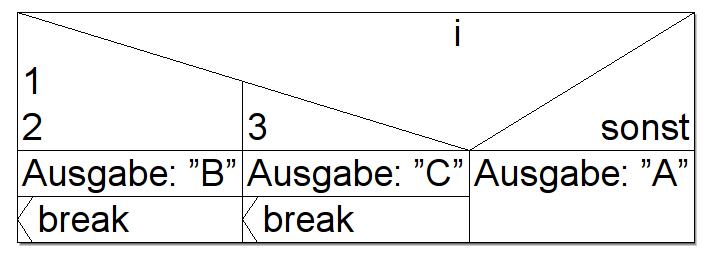
\includegraphics[width=0.6\textwidth]{anweis-2/Bilder/Struktogramm_b}
\end{center}

\end{frame}

\section{Aufgabe 16}
\def\stitle{\theexercise\ - Schleifen 1}
\section{\stitle}
\begin{frame}[t]%
    \frametitle{\stitle}

\lstinputlisting[style=JAVAlines]{schleifen-1/Schleifen1.java}
\begin{itemize}
\item[(a)] Welche Zahl wird auf dem Bildschirm ausgegeben?
\item[(b)] Realisieren Sie diesen Programmausschnitt mit einer \code{while}-Schleife.
\end{itemize}

\end{frame}


\begin{frame}[fragile]%
 \frametitle{a) Starte Programm}%

\begin{description}[style=BASH]
\item[Konsole]
\item javac Schleifen1.java
\item java Schleifen1
\item 0  --  0
\item 1  --  1
\item 2  --  3
\item 3  --  6
\item 5  --  11
\item 6  --  17
\item Ergebnis 17
\end{description}

\end{frame}


\begin{frame}[fragile]%
 \frametitle{b) Als \code{while} Schleife}%

\lstinputlisting[style=JAVAlines]{schleifen-1/Schleifen1_while.java}
\end{frame}

% TODO fix for loop
\section{Aufgabe 17}
\begin{frame}[t]%

\begin{exercise}{Schleifen}
\begin{body}
Gegeben sei der folgende Ausschnitt eines Java-Programms.

\lstinputlisting[style=JAVAlines]{schleifen-2/Schleifen2.java}

\begin{parts}
\item[(a)] Was wird auf dem Bildschirm ausgegeben?
\item[(b)] Realisieren Sie diesen Programmausschnitt mit einer \code{for}-Schleife.
\end{parts}
\end{body}
\end{exercise}
\end{frame}


\begin{frame}[fragile]%
 \frametitle{a) L\"osungsweg}%
\lstinputlisting[style=JAVAlines]{schleifen-2/Schleifen2.java}
\end{frame}


\begin{frame}[fragile]%
 \frametitle{b) Als \code{for} Schleife}%
\lstinputlisting[style=JAVAlines]{schleifen-2/Schleifen2_for.java}
\end{frame}



\begin{frame}
\centering
\Huge\GREEN{Fragen?}
\vspace{2cm}

{\LARGE
N\"achste \"Ubung: 13. November\\
Besprechung Arbeitsblatt 4
}
\end{frame}


%%%%%%%%%%%%%%%%%%%%%%%%%%%%%%%%%%%%%%%%%%%%%%%%%%%%%%%%%%%%%%%%%%%%%%%%
\end{document}
